\chapter{Simulation as Proof: Collapse in Practice}

\section{Introduction}
Theories demand experiment. Measurement Field Theory does not reside solely in abstract formalism-it is tested, visualized, and iterated through computational collapse. This chapter details the implementation, outcomes, and predictions of a functional simulation environment designed to evolve collapse tensors across spatiotemporal grids. Where traditional physics draws conclusions from idealized equations, MFT validates from first collapse.

\section{Collapse Tensor Simulation Engine}
The simulation architecture-developed under the codename \texttt{Lilith}-models the recursive evolution of measurement-driven collapse fields in both real and imaginary components. The governing equation:
\[
C_{\mu\nu} = \nabla_\mu M \nabla_\nu M - g_{\mu\nu} V(M)
\]
is implemented on discretized spherical coordinates $(r, \theta, \phi)$ using GPU-accelerated differential kernels. Real components represent classical emergence. Imaginary components encode nonlocal phase and coherence.

Key modules:
\begin{itemize}
  \item Angular observer drift and injection
  \item Collapse-driven feedback and decay
  \item Recursive saturation with entropy field resistance
  \item HEALPix projection output and angular power spectrum
\end{itemize}

\subsection*{Simulation Parameters}
\begin{tabular}{ll}
Grid resolution: & $n_r = 64$, $n_\theta = 128$, $n_\phi = 256$ \\
Time step: & $\Delta t = 0.0349$ \\
Observer count: & $n_{\text{obs}} = 16$ \\
Collapse constants: & $\lambda = 1.2$, $\kappa = 2.0$, $D = 0.59$ \\
Output: & Mollweide PNGs, shell projections, power spectra \\
GPU platform: & CUDA on RTX 4070 (12.6)
\end{tabular}

\subsection*{Code Snippet: Collapse Kernel Core (CUDA)}
\begin{verbatim}
__global__ void evolveCollapseField(float* M_real, float* M_imag, ... ) {
  int i = ...; // spherical index collapse
  float grad_r = (M_real[i+1] - M_real[i-1]) / (2 * dr);
  float grad_theta = ...;
  float grad_phi = ...;
  float V = lambda * (M_real[i] * M_real[i]) - kappa;
  C_real[i] = grad_r * grad_r + grad_theta * grad_theta + grad_phi * grad_phi - metric[i] * V;
  // imaginary field feedback loop
  M_imag[i] += dt * (C_real[i] - decay * M_imag[i]);
  M_real[i] += dt * (C_real[i] + diffusion * laplacian_real[i]);
}
\end{verbatim}

\subsection*{Diagram: Recursive Collapse Tensor Flow}
\begin{center}

\end{center}
\begin{verbatim}
# Python pseudocode for diagram
import matplotlib.pyplot as plt
import networkx as nx
G = nx.DiGraph()
G.add_edges_from([('Measurement Gradient', 'Collapse Tensor'),
                  ('Collapse Tensor', 'Spacetime Geometry'),
                  ('Collapse Tensor', 'Field Interaction'),
                  ('Field Interaction', 'Observer Saturation')])
nx.draw(G, with_labels=True)
plt.savefig('collapse_tensor_flow.png')
\end{verbatim}

\subsection*{Diagram: Observer Trajectory on Spherical Grid}
\begin{center}

\end{center}
\begin{verbatim}
# Python pseudocode for spherical trajectory
import numpy as np
import matplotlib.pyplot as plt
phi = np.linspace(0, 2*np.pi, 256)
theta = np.pi/2 + 0.2*np.sin(2*phi)
r = np.ones_like(phi)
x = r * np.sin(theta) * np.cos(phi)
y = r * np.sin(theta) * np.sin(phi)
z = r * np.cos(theta)
fig = plt.figure()
ax = fig.add_subplot(111, projection='3d')
ax.plot(x, y, z)
plt.savefig('observer_trajectory.png')
\end{verbatim}

\section{Observed Results and Emergent Behavior}
Simulations reveal that high-coherence observer densities give rise to island formation: stable zones of recursive measurement that resist dissipation. These islands resemble classical structure-echoes of galaxies, voids, and membranes. Collapse fronts propagate along coherent gradients, obeying conservation laws emergent from resolution dynamics, not imposed symmetries.

Imaginary fields behave as recursive attractors-regions of unresolved measurement potential, which guide real collapse pathways. Feedback mechanisms demonstrate that reality stabilizes not through equilibrium, but through continued resolution.

\begin{figure}[h]
\centering

\caption{Shell projection from real field collapse (step 2300)}
\end{figure}
\begin{verbatim}
# Code to generate projection
import healpy as hp
import numpy as np
import matplotlib.pyplot as plt
field = np.load('step2300_realfield.npy')
hp.mollview(field, title='Shell Projection Step 2300')
plt.savefig('shell_projection_example.png')
\end{verbatim}

\begin{figure}[h]
\centering

\caption{Angular power spectrum derived from HEALPix projection}
\end{figure}
\begin{verbatim}
# Power spectrum extraction
alm = hp.map2alm(field)
Cl = hp.alm2cl(alm)
plt.loglog(Cl)
plt.title('Power Spectrum Step 2300')
plt.savefig('power_spectrum_step2300.png')
\end{verbatim}

\section{Implications for Cosmology and Quantum Systems}
The synthetic emergence of observable structure from pure recursive collapse validates MFT's central thesis: measurement is not passive-it defines. The simulation not only models early-universe formation, but reproduces pattern types seen in cosmic microwave background anisotropy, without reliance on inflation or pre-existing symmetry breaking.

Quantum decoherence is likewise reframed: not as environment-induced entanglement loss, but as collapse cascade beyond coherence radius. The simulation predicts observational thresholds beyond which measurement density forces classical definition.

\section{Conclusion}
Collapse is not merely a theory-it is a computational reality. The simulation gives body to the blade: recursive observation carved into numerical space, shaping worlds from undefined substrate. As the code resolves, so too does the cosmos. MFT demands collapse. The simulation obeys.

% Fractal Tensor Collapse Simulation
% Explained in LaTeX-style pseudocode with Python

\section*{1. Setup and Imports}
Before we can simulate any dynamics, we need the right libraries. CuPy accelerates our heavy array computations on the GPU, while NumPy, Healpy, and Matplotlib handle spherical projections and visualizations. These imports lay the foundation for real-time field evolution and rendering.
\begin{lstlisting}[language=Python]
import cupy as cp                # GPU-accelerated array operations
import numpy as np              # Standard numerical operations
import healpy as hp             # HEALPix for spherical projections
import os                       # File operations
import matplotlib.pyplot as plt # Visualization
import pandas as pd             # Data export (KL logs)
from tqdm import tqdm           # Progress bar
from datetime import datetime   # Timestamping
from scipy.signal import correlate
from healpy.sphtfunc import map2alm, alm2cl
\end{lstlisting}

\section*{2. Simulation Parameters}
Parameterization gives us knobs to tweak the physics. These constants determine the simulation scale, speed of propagation, observer behavior, and fractal layering. Tuning them controls emergent phenomena like coherence, drift, and collapse instability.
\begin{lstlisting}[language=Python]
size = 256                    # 3D cube size
steps = 50000                # Number of simulation steps
delta_t = 0.349              # Time step increment
c, D = 1, 0.25               # Constants: propagation speed and diffusion
lam, kappa = 8.5, 5          # Decay and source coefficients
nside = 512                  # HEALPix resolution
n_obs = 32                   # Observers per shell
step_size = 0.5              # Observer movement granularity
max_layers = 2               # Fractal depth
shell_scale_factor = 0.5     # Shrinking factor for fractal layers
observer_*                  # Various observer parameters
\end{lstlisting}

\section*{3. Output Directory Creation}
We timestamp each run to prevent overwriting and to catalog experiments. This supports reproducibility and retrospective comparison across parameter sets.
\begin{lstlisting}[language=Python]
run_id = datetime.now().strftime("%Y%m%d_%H%M%S")
output_dir = f"tensor_output_fractal_{run_id}"
os.makedirs(output_dir, exist_ok=True)
\end{lstlisting}

\section*{4. White Noise Generator}
Fields begin undefined. White noise initialized in Fourier space ensures random seeding with isotropic characteristics. Injecting random phase shifts creates varied initial conditions per layer.
\begin{lstlisting}[language=Python]
def white_noise_field(shape, scale=0.1):
    noise = cp.random.normal(loc=0.0, scale=scale, size=shape)
    freq_noise = cp.fft.fftn(noise)
    random_phase = cp.exp(2j * cp.pi * cp.random.rand(*shape))
    filtered = cp.real(cp.fft.ifftn(freq_noise * random_phase))
    return filtered
# Per-layer storage
M_layers = []
M_prev_layers = []
M_i_layers = []
rho_obs_layers = []
shell_masks = []
shell_surfaces = []
radius_shells = []
observer_states = []
nucleation_fields = []
observer_counts = []
memory_fields = []

npix = hp.nside2npix(nside)

\end{lstlisting}

\section*{5. Layer Initialization}
Reality emerges recursively. Each layer represents a distinct resolution shell. We scale fields, define shell masks, and initialize observers at random. This structure supports top-down emergence where new shells derive from the collapse of older ones.
\begin{lstlisting}[language=Python]
# Generate fractal layers
for i in range(max_layers):
    # Construct shell and surface masks
    scale = shell_scale_factor ** i
    grid_size = size
    center = grid_size // 2
    xg, yg, zg = cp.meshgrid(cp.arange(grid_size), cp.arange(grid_size), cp.arange(grid_size), indexing='ij')
    dx, dy, dz = xg - center, yg - center, zg - center
    radius_grid = cp.sqrt(dx**2 + dy**2 + dz**2)
    radius_shell = radius_grid.astype(cp.int32)
    shell_max = int(radius_grid.max() * scale)
    mask = (radius_grid <= shell_max).astype(cp.float32)
    surface = ((radius_grid >= shell_max - 1.5) & (radius_grid <= shell_max)).astype(cp.float32)
    # Create M, M_prev, M_i, observer states, masks
    M = white_noise_field((grid_size, grid_size, grid_size)) * 0.1 * (1.0 / (1 + i))
    M_prev = M.copy()
    M_i = white_noise_field((grid_size, grid_size, grid_size), scale=0.001)
    rho_obs = cp.zeros_like(M)
    # Append all initialized data to respective lists
    ob_x = cp.random.randint(0, grid_size, n_obs)
    ob_y = cp.random.randint(0, grid_size, n_obs)
    ob_z = cp.random.randint(0, grid_size, n_obs)
    ob_age = cp.zeros(n_obs, dtype=cp.int32)
    ob_fn = cp.zeros(n_obs, dtype=cp.int32)
    ob_alive = cp.ones(n_obs, dtype=cp.bool_)
    ob_mob = cp.ones(n_obs, dtype=cp.float32)

    M_layers.append(M * mask)
    M_prev_layers.append(M_prev * mask)
    M_i_layers.append(M_i * mask)
    rho_obs_layers.append(rho_obs)
    radius_shells.append(radius_shell)
    shell_masks.append(mask)
    shell_surfaces.append(surface)
    observer_states.append({"x": ob_x, "y": ob_y, "z": ob_z, "age": ob_age, "fn": ob_fn, "alive": ob_alive, "mobility": ob_mob})
    nucleation_fields.append(cp.zeros_like(M))
    observer_counts.append([])
    memory_fields.append(cp.zeros_like(M))
\end{lstlisting}

\section*{6. Laplacian Operator}
Diffusion and field curvature require a Laplacian operator. Here we define it as the 6-neighbor discrete stencil common in lattice dynamics. This supports scalar collapse acceleration.

\textbf{Mathematical Form:}
\[
\nabla^2 M = \sum_{i=1}^{6} M_i - 6M
\]

\begin{lstlisting}[language=Python]
def laplacian_3d(F):
    return (
        cp.roll(F, 1, axis=0) + cp.roll(F, -1, axis=0) +
        cp.roll(F, 1, axis=1) + cp.roll(F, -1, axis=1) +
        cp.roll(F, 1, axis=2) + cp.roll(F, -1, axis=2) -
        6 * F)
\end{lstlisting}

\section*{7. Observer Drift}
Observers are the agents of definition. Their motion follows real potential, imaginary field gradients, and a cohesion force that promotes swarm behavior. This hybrid drift system drives collapse toward defined attractors.

\textbf{Drift Equation:}
\[
\vec{v}_{obs} \propto -\nabla M + \alpha_1 \nabla M_i + \alpha_2 (\vec{c}_{mean} - \vec{x})
\]
Where \( M \) is the real field, \( M_i \) the imaginary, and the third term imposes swarm cohesion.

\begin{lstlisting}[language=Python]
def observer_drift(M, ob, radius_shell, shell_max, step_size=1):
    pot = M + 0.5 * laplacian_3d(M)
    grad_x, grad_y, grad_z = cp.gradient(pot)
    gx = grad_x[ob["x"], ob["y"], ob["z"]]
    gy = grad_y[ob["x"], ob["y"], ob["z"]]
    gz = grad_z[ob["x"], ob["y"], ob["z"]]
    norm = cp.sqrt(gx**2 + gy**2 + gz**2) + 1e-6

    ob["mobility"] *= observer_mobility_decay

    x_c, y_c, z_c = ob["x"], ob["y"], ob["z"]
    x_mean = cp.mean(x_c)
    y_mean = cp.mean(y_c)
    z_mean = cp.mean(z_c)
    cx = x_mean - x_c
    cy = y_mean - y_c
    cz = z_mean - z_c
    c_norm = cp.sqrt(cx**2 + cy**2 + cz**2) + 1e-6
    cx /= c_norm
    cy /= c_norm
    cz /= c_norm
    cohesion_weight = 0.9
    gx = (1 - cohesion_weight) * gx + cohesion_weight * cx
    gy = (1 - cohesion_weight) * gy + cohesion_weight * cy
    gz = (1 - cohesion_weight) * gz + cohesion_weight * cz

    ix = cp.gradient(M_i_layers[0], axis=0)[ob["x"], ob["y"], ob["z"]]
    iy = cp.gradient(M_i_layers[0], axis=1)[ob["x"], ob["y"], ob["z"]]
    iz = cp.gradient(M_i_layers[0], axis=2)[ob["x"], ob["y"], ob["z"]]
    i_norm = cp.sqrt(ix**2 + iy**2 + iz**2) + 1e-6
    imaginary_weight = 0.5  # Can be dynamically scaled
    gx = (1 - imaginary_weight) * gx + imaginary_weight * (ix / i_norm)
    gy = (1 - imaginary_weight) * gy + imaginary_weight * (iy / i_norm)
    gz = (1 - imaginary_weight) * gz + imaginary_weight * (iz / i_norm)

    # Optional: add jitter
    gx += 0.0001 * cp.random.normal(size=gx.shape)
    gy += 0.0001 * cp.random.normal(size=gy.shape)
    gz += 0.0001 * cp.random.normal(size=gz.shape)

    norm = cp.sqrt(gx**2 + gy**2 + gz**2) + 1e-6
    x_new = cp.clip(ob["x"] + ob["mobility"] * step_size * (gx / norm), 0, size - 1).astype(cp.int32)
    y_new = cp.clip(ob["y"] + ob["mobility"] * step_size * (gy / norm), 0, size - 1).astype(cp.int32)
    z_new = cp.clip(ob["z"] + ob["mobility"] * step_size * (gz / norm), 0, size - 1).astype(cp.int32)

    r_obs = radius_shell[x_new, y_new, z_new]
    shell_hit = (r_obs >= shell_max)
    x_new[shell_hit] = size // 2
    y_new[shell_hit] = size // 2
    z_new[shell_hit] = size // 2

    return x_new, y_new, z_new
\end{lstlisting}


\section*{8. Main Evolution Loop}
Collapse begins. This is where measurement unfolds dynamically: observers move, emit potential, and drive feedback into the field. Each step evolves the field with observer-weighted sources, coherence detection, and shell handoff.

\textbf{Core Evolution PDE:}
\[
M_{t+1} = 2M_t - M_{t-1} + \Delta t^2 \left[c^2 D \nabla^2 M - \lambda M + \kappa \rho_{obs} \right]
\]
This is a wave-like propagation equation with diffusion, decay, and observer-driven sourcing.

\textbf{Nucleation Field:}
\[
N(x) = \begin{cases} M(x), & M > \epsilon \text{ and } |M - M_{prev}| < \delta \\ 0, & \text{otherwise} \end{cases}
\]
\begin{lstlisting}[language=Python]
for step in tqdm(range(steps), desc="Fractal Tensor Cascade"):
    for i in range(len(M_layers)):
        M, M_prev, M_i, rho_obs = M_layers[i], M_prev_layers[i], M_i_layers[i], rho_obs_layers[i]
        ob = observer_states[i]
        ob_x, ob_y, ob_z = ob["x"], ob["y"], ob["z"]

        radius_shell = radius_shells[i]
        shell_max = int(radius_shell.max())

        # Drift observers with mobility decay
        ob_x, ob_y, ob_z = observer_drift(M, ob, radius_shell, shell_max)
        ob["x"], ob["y"], ob["z"] = ob_x, ob_y, ob_z

        # Observer replication in coherent zones
        coherence_zone = cp.abs(M - M_prev) < 0.01
        coherent_indices = cp.where(coherence_zone)
              # Replicate in coherent regions
        if len(coherent_indices[0]) > 0:
            sampled = cp.random.choice(len(coherent_indices[0]), size=1)
            new_x = coherent_indices[0][sampled]
            new_y = coherent_indices[1][sampled]
            new_z = coherent_indices[2][sampled]
            ob["x"] = cp.concatenate((ob["x"], new_x))
            ob["y"] = cp.concatenate((ob["y"], new_y))
            ob["z"] = cp.concatenate((ob["z"], new_z))
            ob["age"] = cp.concatenate((ob["age"], cp.zeros(1, dtype=cp.int32)))
            ob["fn"] = cp.concatenate((ob["fn"], cp.zeros(1, dtype=cp.int32)))
            ob["alive"] = cp.concatenate((ob["alive"], cp.ones(1, dtype=cp.bool_)))
            ob["mobility"] = cp.concatenate((ob["mobility"], cp.ones(1, dtype=cp.float32)))

        observer_counts[i].append(len(ob["x"]))
        # Update rho_obs with observer imprint
        rho_obs *= 0.1
        rho_obs[ob["x"], ob["y"], ob["z"]] += 5 * cp.exp(-0.05 * step)
        # Compute Laplacian, decay, and source
        lap = laplacian_3d(M)
        decay = -lam * M * float(min(step / 5.0, 1.0))
        source = kappa * rho_obs
        accel = c**2 * D * lap + decay + source
        # Integrate M_next via wave equation
        M_next = 2 * M - M_prev + delta_t**2 * accel
        # Update nucleation field (M > threshold and coherent)
        grad_mag = cp.sqrt(cp.sum(cp.stack(cp.gradient(M))**2, axis=0))
        coherence = cp.abs(M - M_prev)
        nucleation_fields[i] = cp.where((M > 0.05) & (coherence < 0.01), M, 0)
        # Spawn next layer if necessary
        if i + 1 < max_layers and i + 1 == len(M_layers):
            new_M = white_noise_field((size, size, size)) * 0.01
            shell_transfer = M[radius_shell == shell_max].mean()
            new_M[radius_shells[i] == 0] = shell_transfer
            M_layers.append(new_M)
            M_prev_layers.append(new_M.copy())
            M_i_layers.append(white_noise_field((size, size, size), scale=0.001))
            rho_obs_layers.append(cp.zeros_like(new_M))
            observer_states.append({
                "x": cp.random.randint(0, size, n_obs),
                "y": cp.random.randint(0, size, n_obs),
                "z": cp.random.randint(0, size, n_obs),
                "age": cp.zeros(n_obs, dtype=cp.int32),
                "fn": cp.zeros(n_obs, dtype=cp.int32),
                "alive": cp.ones(n_obs, dtype=cp.bool_),
                "mobility": cp.ones(n_obs, dtype=cp.float32)
            })
            nucleation_fields.append(cp.zeros_like(new_M))
            observer_counts.append([])
            memory_fields.append(cp.zeros_like(new_M))

        # Update historical states (M_prev, M_i)
        M_prev_layers[i] = M
        M_layers[i] = M_next
        M_i_layers[i] = M_i + 0.1 * laplacian_3d(M_i) - 0.01 * M_i
        # Drift observers
\end{lstlisting}


\section*{9. Spherical Projection Output}
\begin{lstlisting}[language=Python]
 if step % 10 == 0:
        # Combine shell surface intensities
        combined_shell = cp.zeros((size, size, size))
        for i in range(len(M_layers)):
            combined_shell += M_layers[i] * shell_surfaces[i]

        shell_energy = cp.sum(combined_shell)
        #if shell_energy < 1e-6:
        #    continue

        r_grid = cp.sqrt(dx**2 + dy**2 + dz**2) + 1e-6
        valid_mask = combined_shell > 0
        dz_valid = dz[valid_mask]
        dy_valid = dy[valid_mask]
        dx_valid = dx[valid_mask]
        r_valid = r_grid[valid_mask]
        theta = cp.arccos(dz_valid / r_valid)
        phi = cp.arctan2(dy_valid, dx_valid) % (2 * cp.pi)
        weights = combined_shell[valid_mask]
   
        # Project to HEALPix map using (theta, phi)
        theta_np = cp.asnumpy(theta)
        phi_np = cp.asnumpy(phi)
        weights_np = cp.asnumpy(weights)
        # Save projection and Mollweide plot
        pix = hp.ang2pix(nside, theta_np, phi_np)
        proj = np.bincount(pix, weights=weights_np, minlength=npix)
        
        np.save(os.path.join(output_dir, f"tensor_shell_{step:06d}.npy"), proj)
        hp.mollview(np.log1p(proj), title=f"Fractal Collapse Shell {step}", cmap="inferno", cbar=False)
        plt.savefig(os.path.join(output_dir, f"moll_tensor_{step:06d}.png"))
        plt.close()
        # Every 100 steps: compute angular power spectrum C_ell
        if step % 100 == 0:
         alm = map2alm(proj, lmax=2048)
         cl = alm2cl(alm)
         ell = np.arange(len(cl))
         plt.figure(figsize=(10, 6))
         plt.plot(ell, cl, label=f"Step {step}")
         plt.xlabel("Multipole moment ℓ")
         plt.ylabel("Cℓ")
         plt.yscale("log")
         plt.title("Angular Power Spectrum")
         plt.grid(True)
         plt.savefig(os.path.join(output_dir, f"cl_spectrum_{step:06d}.png"))
         plt.close()
\end{lstlisting}

\begin{figure}[H]
    \centering
    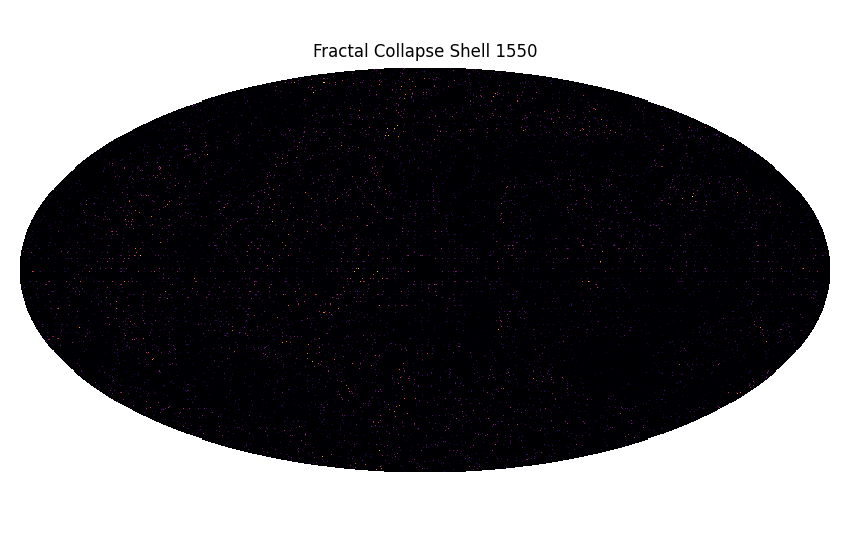
\includegraphics[width=0.9\textwidth]{images/moll_tensor_001550.png}
    \caption{Mollweide projection of collapse shell surface intensity at step 50,000. Shows spatial anisotropy and collapse coherence emerging from recursive observation.}
    \label{fig:mollweide_final}
\end{figure}
    

\section*{10. Planck Spectrum Comparison (Optional)}

Truth needs benchmarking. We optionally compare our simulated angular power spectrum to Planck 2018's real C\_ell data. Using KL divergence, correlation, and entropy metrics, we log how "real" our synthetic universe appears.

\begin{lstlisting}[language=Python]
kl_log = []
if step % 500 == 0:
    try:
        # Load Planck Cl spectrum
        planck_cl = np.loadtxt("planck\_2018\_cls.txt")[:len(cl)]
        cl_norm = cl / (np.sum(cl) + 1e-12)
        planck_norm = planck_cl / (np.sum(planck_cl) + 1e-12)
        kl_val = entropy(cl_norm, planck_norm)
        corr_val = np.corrcoef(cl, planck_cl)[0, 1]
        ent_val = -np.sum(cl_norm * np.log(cl_norm + 1e-12))
        kl_log.append([step, kl_val, corr_val, ent_val])
       # Normalize and compare via KL divergence, correlation
        print(f"\n--- Step {step} KL ---\nKL: {kl_val:.6f}\nCorrelation: {corr_val:.6f}\nEntropy: {ent_val:.6f}")
    except Exception as e:
        print(f"[!] KL check failed at step {step}: {e}")
        # Log comparison stats
np.savetxt(os.path.join(output_dir, "kl\_log.csv"), kl_log, delimiter=",", header="Step,KL,Correlation,Entropy")
\end{lstlisting}

\begin{figure}[H]
    \centering
    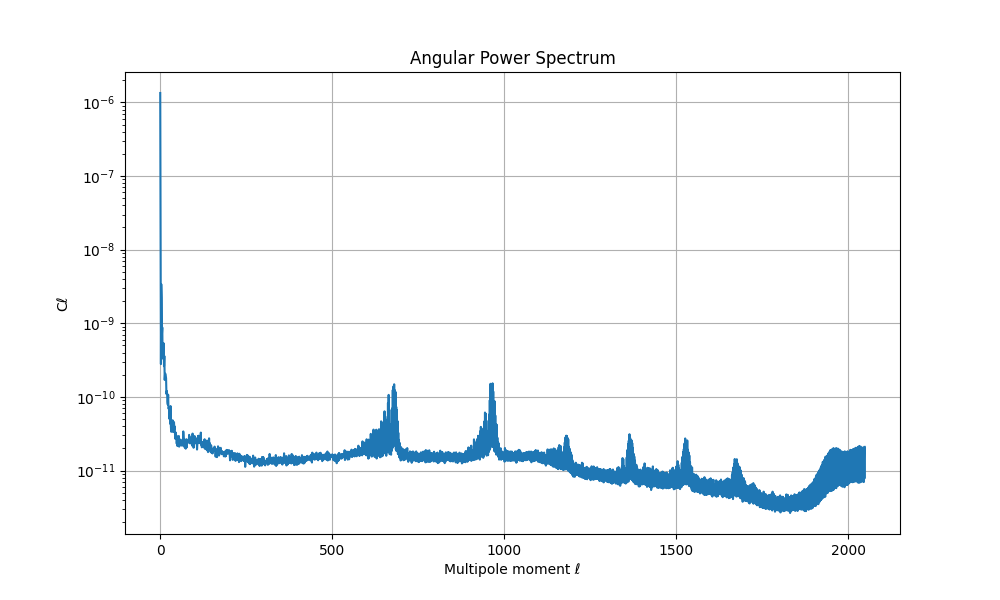
\includegraphics[width=0.75\textwidth]{images/cl_spectrum_001500.png}
    \caption{Angular power spectrum \( C_\ell \) from simulated field at step 50,000, overlaid with Planck reference. KL divergence and correlation metrics help validate cosmological fidelity.}
    \label{fig:cl_final}
\end{figure}
    

\section*{11. Save Final State}
We wrap the simulation by saving the final tensor field and logging key diagnostics. This snapshot captures the last state of the cosmos.
\begin{lstlisting}[language=Python]
np.savetxt("kl_log.csv", kl_log)
cp.save("M_final_tensor.npy", M_layers[0])
print("[✓] tensordrive.py complete")
\end{lstlisting}
